\section{Methods}

\subsection{Problem Formulation}
In crop yield prediction, we denote each county's climatic features by $\mathbf{x}_{c,t}$ and ground-truth crop yield (for a particular crop) by $y_{c,t}\in \mathbb{R}$, where $c$, $t$ represent county and year respectively. Each $\mathbf{x}_{c,t}$ contains four types of features (detailed descriptions of these features can be found in the Experiments section): weather features $\mathbf{x}_{c,t}^w\in \mathbb{R}^{n_w\times 52}$, land surface features $\mathbf{x}_{c,t}^l\in \mathbb{R}^{n_l\times 52}$, soil quality features $\mathbf{x}_{c}^s\in \mathbb{R}^{n_s\times 6}$, and some extra features (e.g. crop production index) $\mathbf{x}_{c}^e\in \mathbb{R}^{n_e}$. Namely, $\mathbf{x}_{c,t}=(\mathbf{x}_{c,t}^w, \mathbf{x}_{c,t}^l, \mathbf{x}_{c}^s, \mathbf{x}_{c}^e)$. We denote the number of weather, land surface, soil quality, and extra variables as  $n_w, n_l, n_s, n_e$ respectively. Among these features, $\mathbf{x}_{c,t}^w, \mathbf{x}_{c,t}^l$ change both spatially and temporally, while $\mathbf{x}_{c}^s, \mathbf{x}_{c}^e$ are county-specific and remain stable over time. The goal is to predict $y_{c,t}$ given $\mathbf{x}_{c,t}$. Recent work \cite{khaki2020cnn} also showed features from past years can help with the prediction, so we reformulate our task as predicting $y_{c,t}$ with $\{\mathbf{x}_{c,t},\mathbf{x}_{c,t-1},...,\mathbf{x}_{c,t-\Delta t}\}$. $\Delta t$ is the length of year dependency. If $\Delta t=0$, the model will not consider features from prior years. 

\subsection{Per-Year Embedding Extraction}
Regardless of whether the models use historical features or not, the first step is always to extract an embedding for each year from $\mathbf{x}_{c,t}$. Then a prediction can be made based on the embedding from the current year or the embeddings from the last few years.

The four types of features $\mathbf{x}_{c,t}^w, \mathbf{x}_{c,t}^l, \mathbf{x}_{c}^s, \mathbf{x}_{c}^e$ have different structures. Using a uniform neural network to extract the embedding may not effectively exploit the structure in the raw data. For example, weekly features $\mathbf{x}_{c,t}^w, \mathbf{x}_{c,t}^l$ naturally incorporate a temporal order, but county-specific soil features $\mathbf{x}_{c}^s$ do not change temporally and are measured at different depths underground. Therefore, we use separate neural networks to process the differently structured-parts from $\mathbf{x}_{c,t}$:
\begin{equation}
\label{eq:cnn}
\begin{aligned}
&\mathbf{h}_{c,t}^{wl}=f_{wl}(\mathbf{x}_{c,t}^w, \mathbf{x}_{c,t}^l) \\
&\mathbf{h}_{c}^s=f_s(\mathbf{x}_{c}^s) \\
&\mathbf{h}_{c,t}=(\mathbf{h}_{c,t}^{wl}, \mathbf{h}_c^s, \mathbf{x}_{c}^e)
\end{aligned}
\end{equation}
$f_{wl}(\cdot)$ handles the features that vary over time. Since land surface features like soil moisture from $\mathbf{x}_{c,t}^l$ are weekly data closely related to weather, we concatenate $\mathbf{x}_{c,t}^l$ and $\mathbf{x}_{c,t}^w$ before further passing to $f_{wl}$. Given the temporal order, an RNN or a CNN can be used for $f_{wl}$ to facilitate information aggregation along the time axis. On the other hand, $f_s(\cdot)$ aggregates information along soil depths. We use CNN as the architecture for $f_s$. $\mathbf{x}_{c}^e$ only contains six scalar values, so we directly pass it to the output embedding. The final embedding $\mathbf{h}_{c,t}$ is the concatenation of $\mathbf{h}_{c,t}^{wl}, \mathbf{h}_c^s, \mathbf{x}_{c}^e$.


\begin{figure*}[t]
\centering
\begin{minipage}[c]{7cm}
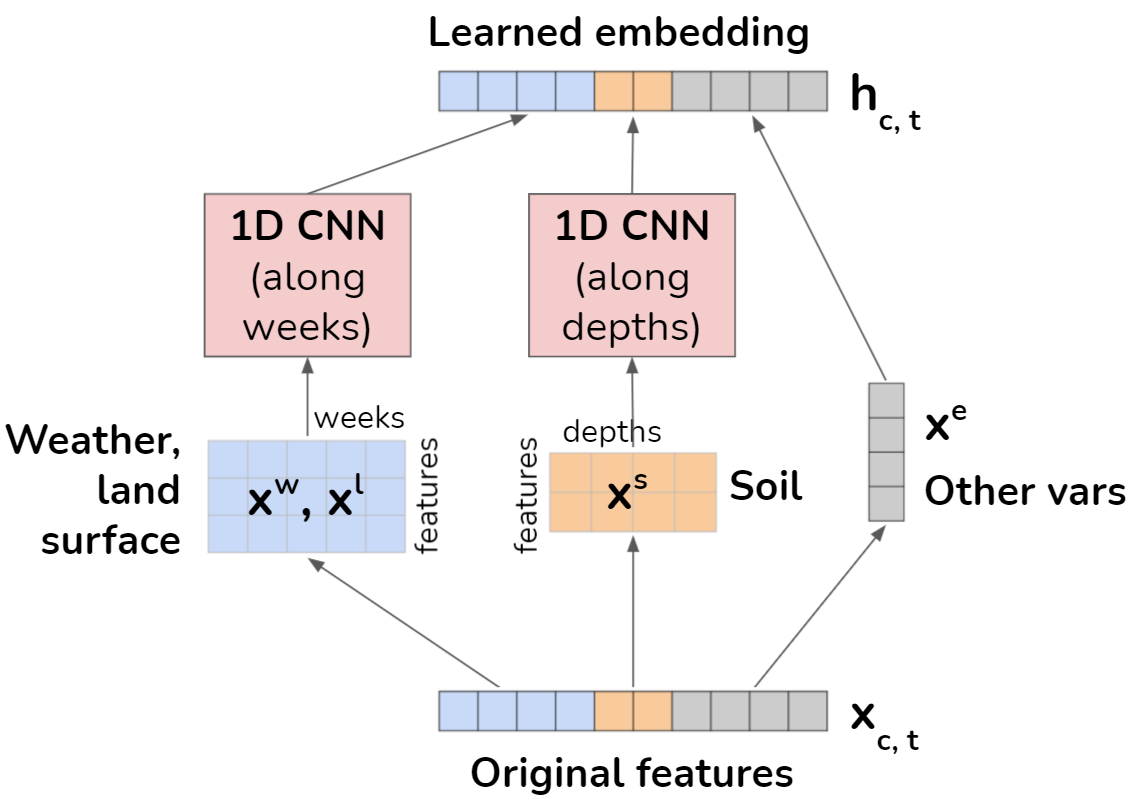
\includegraphics[width=6.9cm]{figs/cnn.png}
\label{fig:cnn}
\end{minipage}
\begin{minipage}[c]{10cm}
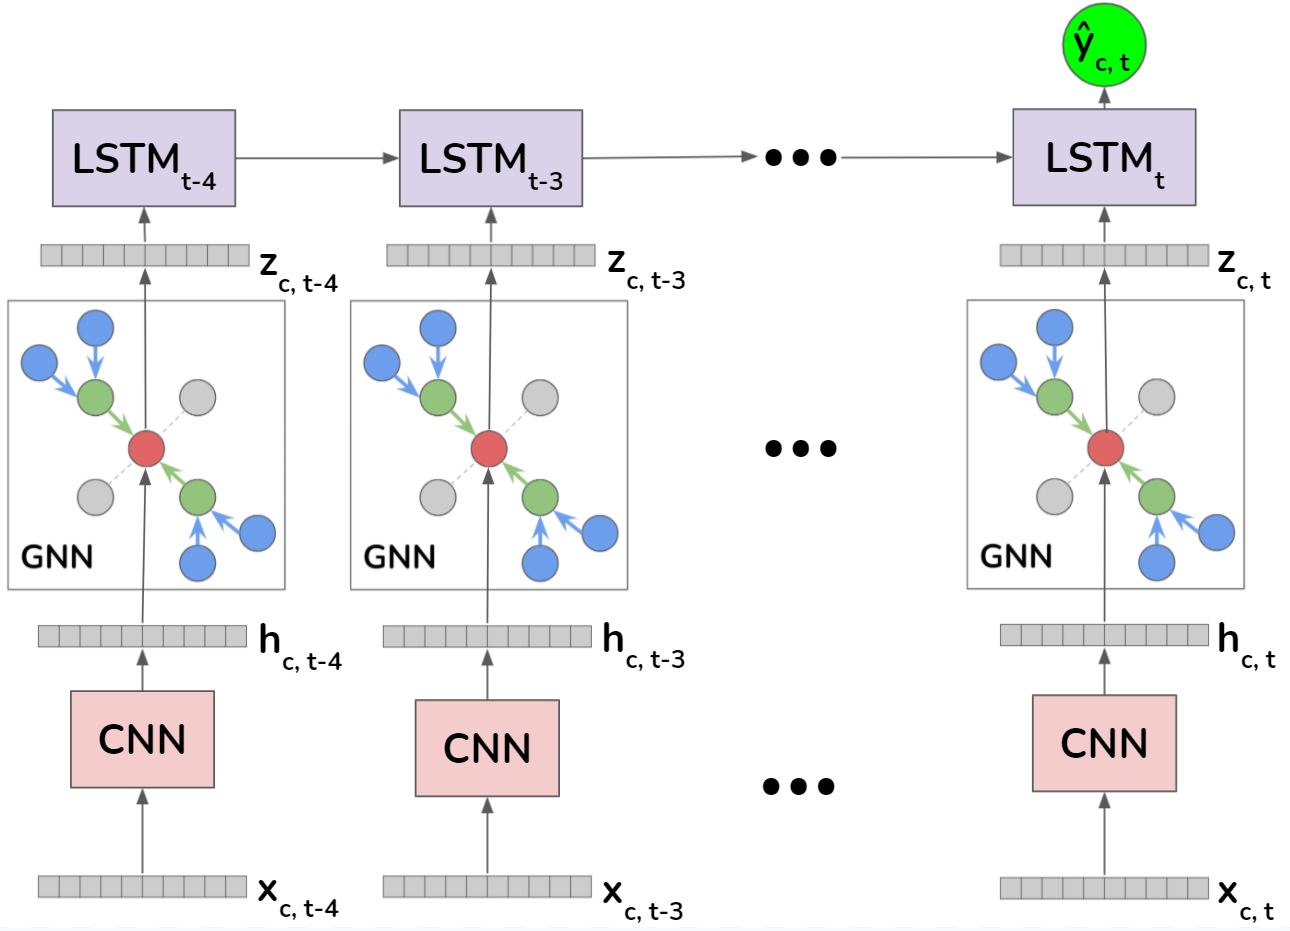
\includegraphics[width=9.9cm]{figs/gnn-rnn.png}
\label{fig:gnn-rnn}
\end{minipage}
\caption{\textbf{Left}: The CNN model used for per-year embedding extraction. \textbf{Right}: Our overall GNN-RNN framework. For each county $c$ and year $t'$, the CNN extracts an embedding $\mathbf{h}_{c, t'}$. Then we apply a GNN to refine each year's embedding by aggregating information from neighboring counties, producing a new embedding $\mathbf{z}_{c, t'}$. Finally, an LSTM processes the embeddings from each year and outputs the yield prediction $\widehat{y}_{c, t}$.}
\end{figure*}


\subsection{Temporal Dependency}
Though new crops are planted every year and yields primarily depend on climatic factors within one year, it has been observed that the trend and variations captured by recent history can be very informative for prediction \cite{khaki2020cnn}. For example, crop yields have tended to increase over the past few decades due to improvements in technology and genetics \cite{ortiz2018another}. While data on the underlying technological improvement is unavailable \cite{khaki2020cnn}, we can observe recent trends in crop yield. Our per-year embedding extraction makes it easy to incorporate  historical knowledge. All we need is an RNN that reads the per-year embeddings from the current year and several prior years. The output from the last time step would be our prediction for the crop yield of the current year: 
\begin{equation}
\label{eq:rnn}
\begin{aligned}
\widehat{y}_{c,t}=r(\mathbf{h}_{c,t-\Delta t}, ..., \mathbf{h}_{c,t-1}, \mathbf{h}_{c,t})
\end{aligned}
\end{equation}
where $r(\cdot)$ is an RNN, and $\mathbf{h}_{c,t'}$ is the embedding from year $t'$ for county $c$. The model described so far follows the CNN-RNN framework, which has previously been shown to outperform single-year NN models \cite{khaki2020cnn}.


\subsection{Incorporating Geographical Knowledge}
Eq.~\ref{eq:rnn} shows how one can extend the use of embeddings from Eq.~\ref{eq:cnn} temporally. Then a natural question is, Can we take advantage of the embeddings geospatially as well? Intuitively, if a county has good yields, nearby counties tend to have good yields as well. The weather and soil conditions should also transition smoothly across the continent. The additional features from neighboring counties could boost the prediction if used properly. A recent success in COVID-19 forecasting \cite{kapoor2020examining} with similar insights could further support incorporating geographical knowledge, where the graph-based representation learning greatly improves case prediction. 

\subsubsection{Graph Neural Network}
Graph Neural Network (GNN) \cite{zhou2020graph} is a novel type of neural network proposed to unravel the complicated dependencies inherent in graph-structured data sources.
%GNN allows more flexibility and a wider representation space to embed the node and edge information from the graph for inference.
Given its strong power in representation learning, GNN has demonstrated prominent applications in chemistry \cite{gilmer2017neural}, traffic \cite{cui2019traffic}, biology \cite{fout2017protein}, and computer vision \cite{satorras2018few} with sophisticated model architectures \cite{kipf2016semi,hamilton2017inductive,velivckovic2017graph}. Formally, a graph is denoted by $G=(V,E)$ where $V$ is the set of nodes and $E$ is the set of edges between nodes. In our crop yield prediction task, each node is a county. $E$ is represented as a symmetric adjacency matrix $A\in \{0,1\}^{N\times N}$ where $A_{i,j}=1$ if two counties $v_i, v_j\in V$ border and $A_{i,j}=0$ otherwise. $N$ is the total number of counties. Each node is associated with $\mathbf{x}_{c,t}$ for every year. 

\subsubsection{GraphSAGE} 
A popular GNN model, GraphSAGE, \cite{hamilton2017inductive} is a general framework that leverages node feature information and learns node embeddings through aggregation from a node's local neighborhood. Unlike many other methods based on matrix factorization and normalization \cite{jia2020residual}, GraphSAGE simply aggregates the features from a local neighborhood, and is thus less computationally expensive. The features can be aggregated from a different number of hops or search depth. Therefore the model often generalizes better. GraphSAGE is suitable for crop yield prediction because most counties only border a few others and the adjacency matrix is sparse. It also provides flexible aggregation methods.

Formally, for the $l$-th layer of GraphSAGE, 
\begin{equation}
\label{eq:gnn}
\begin{aligned}
&\mathbf{a}_{c,t}^{(l)} = g_l(\{\mathbf{z}_{c',t}^{(l-1)},\forall c'\in\mathcal N(c)\})\\
&\mathbf{z}_{c,t}^{(l)} = \sigma(\mathbf{W}^{(l)}\cdot (\mathbf{z}_{c,t}^{(l-1)}, \mathbf{a}_{c,t}^{(l)}))
\end{aligned}
\end{equation}
where $\mathbf{z}_{c,t}^{(0)}=h_{c,t}$ from Eq.~\ref{eq:cnn}, and $l\in\{0,1,...,L\}$. $\mathcal N(c)=\{c', \forall A_{c,c'}=1\}$ is the set of neighboring counties for $c$. The aggregation function for the $l$-th layer is denoted $g_l(\cdot)$, which could be mean, pooling, or graph convolution (GCN) function. In practice, we found mean or pooling are effective and computationally efficient. $\mathbf{a}_{c,t}^{(l)}$ is the aggregated embedding from the bordering counties. We concatenate $\mathbf{a}_{c,t}^{(l)}$ with the last layer's embedding $\mathbf{z}_{c,t}^{(l-1)}$ before the transformation using $\mathbf{W}^{(l)}$. $\sigma(\cdot)$ is a non-linear function.

\subsubsection{GNN-RNN}
The output embedding from GNN's last layer $\mathbf{z}_{c,t}^{(L)}$ thus extracts the information (e.g., weather, soil) from the whole local neighborhood for year $t$. To integrate the historical knowledge, we can do the same as in Eq.~\ref{eq:rnn}, by taking the GNN output embeddings from prior years:
\begin{equation}
\label{eq:gnn-rnn}
\begin{aligned}
\widehat{y}_{c,t}=r(\mathbf{z}_{c,t-\Delta t}^{(L)}, ..., \mathbf{z}_{c,t-1}^{(L)}, \mathbf{z}_{c,t}^{(L)})
\end{aligned}
\end{equation}
where $\mathbf{z}_{c,t'}^{(L)}$ is the GNN embedding from year $t'$.

\subsubsection{Loss Function}
We use log-cosh function as our objective:
\begin{equation}
\begin{aligned}
L(\widehat{y}_{c,t}, y_{c,t})=\log(\text{cosh}(\widehat{y}_{c,t}-y_{c,t}))
\end{aligned}
\end{equation}
Log-cosh works similarly to mean square error, but is not as strongly affected by the occasional wildly incorrect prediction. It is also twice differentiable everywhere. Mini-batch training is adopted during optimization. Batch loss is the average log-cosh loss of all samples in a batch. 
